\subsection{Ciona as a model}
	The ascidian \textit{Ciona intestinalis}, a marine invertebrate animal, has a long history in developmental biology and evoutionary biology. 
	Darwin highlighted the importance of the ascidians due to their  close phylogenetic relationship to the vertebrates (REF). 
	Also, it provided one of the first evidences of localized determinants of cell specification (Conklin, 1905). 
	Although their adult form is a sessile filter feeder, its tadpole larva has characteristic features of the chordate group: a dorsal neural tube, a notochord surrounded by muscle and a ventral endodermal strand (Satoh, 1994).
	Ascidians show morphogenetic movements during gastrulation and neurulation similar to vertebrates and both share common genetic regulators of cell specification (REF).
	Their relative short life cycle, almost transparent body and rapid development facilitate many genetic techniques and are partly responsible for the re-emergence of \textit{C. intestinalis} as model organism in developmental biology (REF, Levine). 

\subsection{Current knowledge about Ciona development}
	The sequencing of the \textit{C. intestinalis} genome (Dehal, 2002) facilitated its comparison with other vertebrate sequenced genomes and the analysis of gene expression through its life cycle.
	The \textit{C. intestinalis} genome is only 160Mb and contains ~16,000 genes, a gene number similar to the invertebrate \textit{D. melanogaster} genome and only is half of the genes found in some vertebrates (REF).
	This low number of genes (compared to vertebrates) can be explained by the finding that many gene families or subfamilies have only one representative in \textit{C. intestinalis} (Dehal, 2002).
	Relevant efforts have been made to describe the spatial expression patterns of individual genes (REF).
	The spatial expression patterns of  >1,000 cDNA clones have been described using whole-mount in situ hybridization techniques at different developmental stages (REF).
	 Importantly, the developmental stages included cover a wide temporal range, e.g., blastula, gastrula and tapole stages (REF).
	 Taking advantage of the ascidian invariant cleavage pattern and well described lineage analysis (Conklin, Nishida 1987), the cDNA spatial expression have been described at the single cell level up to the early gastrula stage (REF), making this database an invaluable resource to investigate the spatio-temporal dynamics of gene expression.





Start with some text.
\begin{figure}[h]
  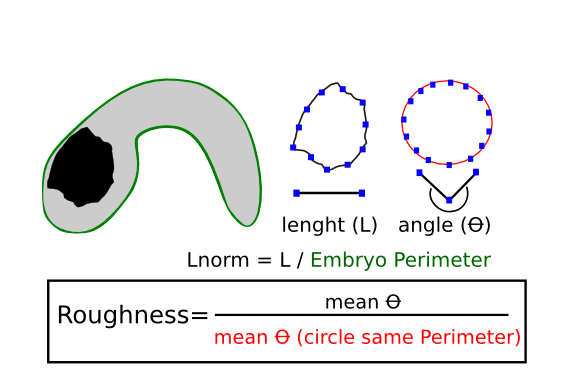
\includegraphics[width=6cm]{./Images/Fig.png}
  \centering
  \caption{This is a figure caption}
  \label{fig:Fig}
\end{figure}


Figure \ref{fig:Fig} shows an example on how figures in the 
png format can be included into the text.\par